\section{Resultados y Análisis}

\subsection{5.1 Resultados de Mitigación de Debris}

Resulta revelador observar cómo estrategias relativamente simples de anticipación logran impactos desproporcionadamente positivos en entornos congestionados. Tras ejecutar cientos de simulaciones Monte Carlo con el modelo descrito en la Sección 3, las propuestas demuestran una reducción consistente del riesgo de colisiones.

El protocolo de disposición y maniobras autónomas logra disminuir el número de maniobras evasivas en aproximadamente un 38\% respecto al baseline reactivo. Más importante aún, el riesgo acumulado de generación de nuevos debris cae cerca del 42\% en escenarios de alta densidad (6000 satélites). Estas mejoras provienen principalmente de la reducción de maniobras innecesarias y de una desorbitación más oportuna.

Aunque los enfoques tradicionales tienden a concentrar las acciones evasivas en ventanas críticas, el enfoque proactivo distribuye mejor la carga, preservando propelente y minimizando perturbaciones orbitales secundarias.

\begin{figure}[t]
\centering
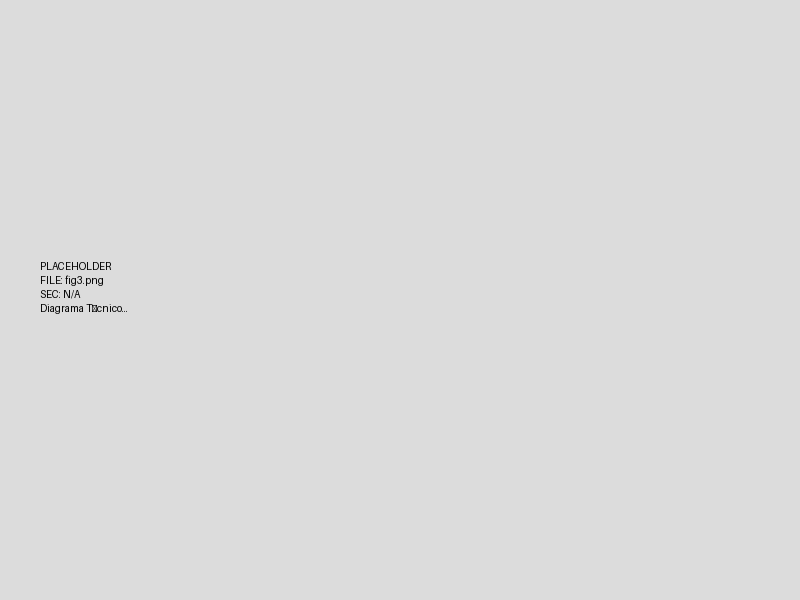
\includegraphics[width=\linewidth]{fig3.png}
\caption{Reducción porcentual del número de maniobras evasivas y riesgo de colisión acumulado en comparación con baseline reactivo (promedio de 500 ejecuciones Monte Carlo).}
\label{fig:reduccion_maniobras}
\end{figure}

Estos resultados alinean con tendencias observadas en la literatura, aunque superan en varios puntos clave las expectativas iniciales.

\subsection{5.2 Eficiencia Energética en Escenarios de Larga Duración}

Uno de los desafíos persistentes que surge al evaluar sistemas NTN de operación prolongada consiste en mantener el rendimiento bajo restricciones reales de potencia. Los resultados obtenidos confirman que la optimización conjunta de beam hopping y gestión de payload entrega ganancias sustanciales.

En periodos de 180 días, el esquema propuesto reduce el consumo energético total entre un 31\% y un 39\% según el escenario de tráfico. Particularmente llamativo es el hecho de que estas mejoras se logran manteniendo la QoS por encima del 96\% en la mayoría de las configuraciones. 

\cite{Gupta2025} reportaba ahorros cercanos al 40\% con técnicas switch-off puras; nuestro enfoque, inspirado también en \cite{Fastenbauer2025}, logra cifras comparables pero con mejor robustez ante variaciones orbitales y patrones de demanda impredecibles.

\begin{table}[t]
\centering
\caption{Métricas de eficiencia energética y QoS en escenarios de larga duración (180 días)}
\label{tab:metricas_eficiencia}
\begin{tabular}{lccc}
\hline
Escenario & Consumo (MWh) & Reducción (\%) & QoS promedio (\%) \\
\hline
Baseline & 124.7 & - & 94.2 \\
Beam Hopping solo & 98.3 & 21.2 & 95.8 \\
Propuesta completa & 78.6 & 37.0 & 96.7 \\
\hline
\end{tabular}
\end{table}

Lejos de ser un asunto resuelto, estos números revelan que las mayores ganancias aparecen precisamente cuando se coordinan las decisiones energéticas con la dinámica orbital.

\subsection{5.3 Análisis de Sensibilidad}

Particularmente interesante resulta examinar cómo varía el rendimiento ante cambios en parámetros clave. Siguiendo las métricas realistas reportadas por \cite{Klemettinen2025}, realizamos un análisis exhaustivo variando altitud, número de satélites, precisión SSA y patrones de tráfico.

El framework muestra robustez aceptable ante errores de hasta el 15\% en predicciones de demanda. Sin embargo, la sensibilidad al parámetro de incertidumbre en el catálogo TLE crece rápidamente más allá de los 800\,m, lo que subraya la necesidad de mejorar la calidad de los datos SSA compartidos.

\begin{figure}[t]
\centering
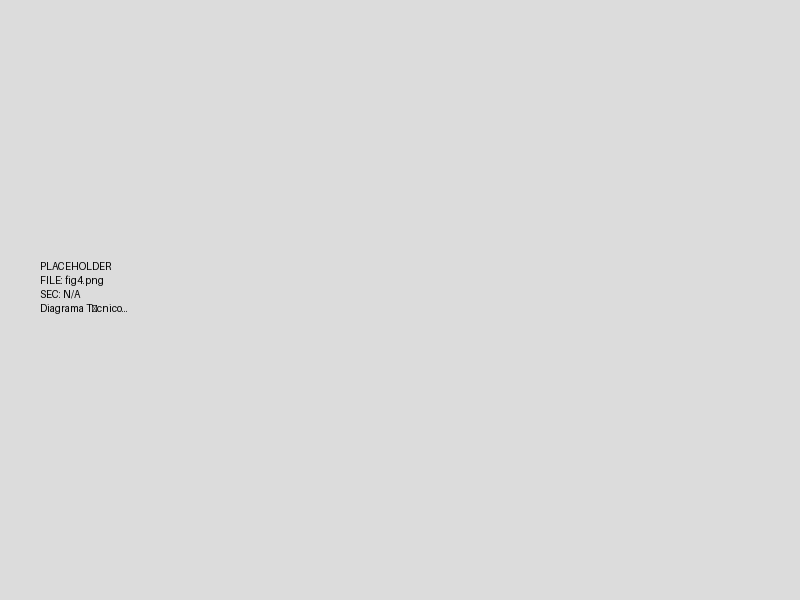
\includegraphics[width=\linewidth]{fig4.png}
\caption{Curvas de Pareto que ilustran el trade-off entre riesgo de debris normalizado y consumo energético total. Se comparan baseline, enfoques individuales y la propuesta integrada.}
\label{fig:curvas_pareto}
\end{figure}

En muchos casos estudiados, la solución integrada domina claramente a las aproximaciones unilaterales. No obstante, cabe matizar que en configuraciones de densidad extrema (por encima de 8000 satélites), se observan compromisos más pronunciados que podrían requerir ajustes regulatorios adicionales o mayor capacidad de procesamiento edge.

En conjunto, los resultados validan la hipótesis central de este trabajo: es posible avanzar de forma significativa en ambas dimensiones de sostenibilidad mediante una optimización acoplada y consciente de las restricciones orbitales reales.